%BeginFileInfo
%%Publisher=TEMP
%%Project=VYTAS
%%Manuscript=AICOM2E
%%Stage=100
%%TID=Vytas
%%Format=latex
%%Distribution=live
%%Destination=PDF
%%DVI.Maker=vtex_tex_dvi
%%PDF.Maker=live_tex_pdf
%%DVX.Maker=vtex_tex_dvx
%%Compiler cmd line=LATEX612.BAT %N.TEX
%EndFileInfo
% Journal: Applied Ontology, IOS Press
% Latex 2e
% Test file ao2e.tex
%
\documentclass[jou]{ao2e}%[seceqn,secfloat,secthm]

\usepackage[T1]{fontenc}
\usepackage{times}%
\usepackage{natbib}
\usepackage{moreverb}
\usepackage[nolist]{acronym}
\usepackage{url}
%\usepackage{pdftex} 
\usepackage{graphicx} 

\newcommand{\protege}{Prot\'{e}g\'{e}}
%\usepackage{todonotes}

%\firstpage{1}
%\lastpage{3}
%\volume{3}
%\pubyear{2009}

\begin{document}
\begin{frontmatter}                           % The preamble begins here.
%
%\pretitle{Pretitle}
\title{ MIREOT: the Minimum Information to Reference an External Ontology Term}
\runningtitle{MIREOT: the Minimum Information to Reference an External Ontology Term}
%\subtitle{Subtitle}

\author[A]{\fnms{M\'elanie} \snm{Courtot}%
\thanks{Corresponding author: M\'elanie Courtot, BC Cancer Agency, Vancouver, BC, Canada.}},
\author[B]{\fnms{Frank} \snm{Gibson}},
\author[C]{\fnms{Allyson L.} \snm{Lister}},
\author[D]{\fnms{James} \snm{Malone}},
\author[E]{\fnms{Daniel} \snm{Schober}},
\author[A]{\fnms{Ryan R.} \snm{Brinkman}}
and
\author[F]{\fnms{Alan} \snm{Ruttenberg}}

\runningauthor{M. Courtot et al.}
\address[A]{BC Cancer Agency, Vancouver, BC, Canada\\
E-mail: mcourtot@gmail.com, rbrinkman@bccrc.ca}

\address[B]{Abcam plc, 332 Cambridge Science Park, Cambridge, CB4 OWN, UK\\
E-mail: fgibson@gmail.com}

\address[C]{CISBAN and School of Computing Science, Newcastle University, Newcastle upon Tyne, UK\\
E-mail: a.l.lister@newcastle.ac.uk}

\address[D]{The European Bioinformatics Institute, Cambridge, CB10 1SD, UK\\
E-mail: malone@ebi.ac.uk}

\address[E]{Institute of Medical Biometry and Medical Informatics (IMBI), University Medical Center, 70104 Freiburg, Germany\\
E-mail: schober@imbi.uni-freiburg.de}

\address[F]{Science Commons, Cambridge, MA, USA\\
E-mail: alanruttenberg@gmail.com}


\begin{abstract}
While the Web Ontology Language (OWL) provides a mechanism to import ontologies, this mechanism is not always suitable.
Current editing tools present challenges for working with large ontologies and direct OWL imports can prove impractical for day-to-day development.
Furthermore, external ontologies often undergo continuous change which can introduce conflicts when integrated with multiple efforts.
Finally, importing heterogeneous ontologies in their entirety may lead to inconsistencies or unintended inferences.
In this paper we propose a set of guidelines for importing required terms from an external resource into a target ontology.
We describe the methodology, its implementation, present some examples of this application, and outline future work and extensions.
\end{abstract}


\begin{keyword}
ontology import\sep data integration\sep MIREOT
\end{keyword}

\end{frontmatter}

\section{Introduction}

The ability to share and reuse existing ontological resources is an important consideration when developing a new ontology.
For example, when developing an ontology related to the biomedical domain, it may be useful to include terms from the \ac{GO}~\citep{GO} to represent biological processes or from the \ac{PATO}~\citep{PATO} to represent properties of entities.
Ontologies such as GO and PATO are built collaboratively by communities of experts and are the products of substantial effort; recapitulating this work instead of reusing it represents a duplication of development effort and results in multiple ontologies covering the same domain. It could also result in projects having different unique identifiers to denote the same entity, which would require post-hoc, potentially error-prone, identifier mapping systems to enable data integration. 
While it appears that building upon existing vocabularies is the best way to proceed, ontology developers are faced with a number of practical challenges when trying to do so.
The easiest way to integrate an existing body of work is to rely on the \ac{OWL}~\citep{OWL} mechanism \emph{owl:imports}, which imports the external resource as a whole.
However, current limitations in tools and reasoners can sometimes make this impractical.
Popular OWL tools (\emph{e.g.}, Prot\'eg\'e~\citep{Protege} and Pellet~\citep{Sirin}) can neither load nor reason over very large ontologies such as the NCBI Taxonomy~\citep{NCBI} or the Foundational Model of Anatomy~\citep{FMA}, making direct \ac{OWL} imports of such resources impractical. 
Furthermore, external ontologies may have been constructed using design principles which do not align with the practice of the ontology requiring their import.  In this instance, wholly importing such ontologies could lead to inconsistencies or unintended inferences. 
Other import options are possible, for instance using software that extracts a \emph{module}~\citep{Grau} of the external ontology.
A module can be seen as a fragment of an external ontology that, when imported by an other ontology, allows the same inferences to be drawn with respect to the classes of interest as if the whole ontology had been imported. This solution allows developers to pick only pieces of the source ontology (and thus overcome size issues) without losing any reasoning power.
However, if an extracted module is to be useful, the external ontology needs to be structured in a way that is compatible with the importing ontology (\emph{e.g.}, using the same upper ontology and relationship types), and the logical axioms need to be accurate. 
This is not always the case at the current stage of development of some resources.
For example, during the development of the \ac{OBI}~\citep{OBI}, importing the root class of the \ac{CARO}~\citep{CARO} was not desired as its definition intersected multiple classes in \ac{OBI}, making it difficult to determine how the two ontologies aligned.
In addition, although software that extracts modules are available, most are only in early stages of development.

We tried several modularization tools~\citep{Grau2, Jimenez,Seidenberg,Sirin}. 
All of them discarded annotations, resulting in modules containing only the class declarations and no annotation properties, such as labels or definitions.
We also experienced software crashes on large ontologies (the size of the ontologies capable of being loaded varying with the tool; for example we were able to load the \ac{ChEBI} Ontology~\citep{ChEBI} with SWOOP but not with Prot\'eg\'e 3.4).
One tool~\citep{Seidenberg} had undocumented assumptions about the form of URIs used as class names and therefore extracted empty modules. 
The other tools described were able to extract modules by automatically determining their size. This resulted in either a single term or a large number of terms being extracted, depending on the provided arguments, as the tools attempt to approximate a module without discarding potentially useful information. These large modules undermine the goal of having imports of a manageable size.
Our conclusion was that the current ontology modularization tool set is in the early stages of development and, though promising, does not address our current needs.

To address these issues we developed a set of guidelines for importing terms from multiple resources, avoiding the overhead of importing the complete ontology from which the terms derive. 
The \ac{MIREOT} guidelines were created to aid the development of \ac{OBI}.
\ac{OBI} uses the \ac{BFO}~\citep{BFO} as an upper-level ontology and has been submitted for inclusion in the \ac{OBO} Foundry~\citep{OBOFoundry}. 
One of the fundamental principles of the \ac{OBO} Foundry is to reuse, where appropriate, existing ontology resources, therefore avoiding duplication of effort and ensuring orthogonality.
\ac{MIREOT} provides a mechanism by which external ontology terms can be selectively imported, even if they do not use a particular upper ontology or OWL DL~\citep{Horrocks}, and hence contribute to the realization of OBO Foundry principles.

\section{Policy}

In deciding upon a minimum unit of import, our first step was to consider the practice of other ontology efforts.
For example, in the \ac{GO}, the intended denotation of classes remains stable such that even when the ontology is repaired or reorganized, the effects of such changes do not affect the intended meaning of individual terms.
Rather, the changes are towards more carefully expressing the logical relations between them.
When a term's changes meaning, the term is deprecated~\citep{GOGuide}.
We can therefore consider a term as stable, in isolation from the rest of the ontology, and use terms (\emph{i.e.}, individual classes in isolation from the ontology) as basic unit of import.
The current implementation of \ac{MIREOT} has been limited to import of terms from other ontologies that aspire to the OBO Foundry, and so adhere to a similar deprecation policy.
The minimum amount of information needed to reference an external term is its \ac{URI} (\textit {i.e.}, the identifier for this term) and its source ontology \ac{URI} (\textit {i.e.}, where the term comes from). 
Generally, these items remain stable and can be used to unambiguously reference the external term.
The minimum amount of information to then integrate this class in the importing target ontology is its desired position in the hierarchy, specifically the URI of its direct superclass (\textit {i.e.}, under which class the term is to be asserted).

Taken together, the following minimal set is enough to consistently reference an external term:
\begin{itemize}
 \item \textbf{source ontology \ac{URI}} The logical \ac{URI} of the ontology containing the external term to be imported. 
 \item \textbf{source term \ac{URI}} The logical \ac{URI} of the specific term to import. 
 \item \textbf{target direct superclass \ac{URI}} The logical \ac{URI} of the direct asserted superclass in the importing ontology.
\end{itemize} 

To ease development of the importing ontology it is also recommended, although not required, that additional information about the external class be added, such as its label and textual definition, or any other kind of information that may be deemed useful by the ontology developers.
This additional information, when appropriate, is mapped into the importing ontology's annotation properties. As it is prone to modification by the source ontology developers (\textit{e.g.}, when updating a definition), it is stored in a separate file that can be removed and rebuilt on a regular basis, allowing for regular update within the importing target ontology.


\section{Implementation}

An implementation of the \ac{MIREOT} guidelines was performed in the context of the \ac{OBI} project, and can be decomposed into a two-step process:

\begin{enumerate}
\item Gather the minimum information for the external class.
\item Use this minimum information to fetch additional elements, like labels and definitions.
\end{enumerate}

Once the external term is identified for import, the first step is to gather the corresponding minimum information set.
This set is stored in a file called \emph{external.owl} (all scripts and files are available under the \ac{OBI} Subversion Repository~\citep{OBIScripts}).
In the current implementation, a Perl script, \emph{add-to-external.pl}, can be used to append the minimum information set for a given external term to the \emph{external.owl} file.
The script takes as arguments the identifier of the external class to be imported and its parent class in the target hierarchy.
In addition, a mapping between the prefix used in the identifier and the external source ontology \ac{URI} is built into the script. For example, when requesting the term \textit{CL:0000767} (see below), the script maps the \textit{CL:} prefix to its source ontology \ac{URI} \url{http://purl.org/obo/owl/CL}.
Curators therefore need only specify the ID of the external class to import (rather than the full URI) and the ID of the class it should be imported under.
Upon addition of an external class, a visual check can be performed as the perl scripts returns the \ac{OWL} excerpt added to the file to the user.

In the current implementation, the additional information can be obtained programmatically via SPARQL~\citep{SPARQL} CONSTRUCT queries (Figure \ref{fig:sparql}).
These queries~\citep{OBIQueries} specify, for each source ontology, which extra elements about the term is to be extracted, such as the definition and preferred label, and how to map these into the corresponding OBI annotation properties. 


\begin{figure}[t]
\scriptsize
\verbatiminput{./figs/sparql.txt} 
\caption{Template SPARQL query. For convenience, we use alias:preferredTerm and
alias:definition to reference our annotations properties IAO\_0000111 and IAO\_0000115~\citep{IAO} respectively. The \_ID\_GOES\_HERE\_ pattern will be replaced by the script when building the CONSTRUCT query.}
\label{fig:sparql}
\end{figure}

For example, in the current \ac{OWL} rendering of \ac{OBO} files, definitions are individuals and the rdfs:label of those individuals record the text of the definitions. 
Within the \ac{OBI} implementation of the \ac{MIREOT} guidelines, the value of the rdfs:label of the oboInOwl:Definition will be set to the value of \url{http://purl.obolibrary.org/IAO_0000115} (\emph{i.e.,} iao:definition). Only annotation properties which map directly to the target ontology's own metadata are copied; new properties, if not specified in the source ontology, are not created. 

Finally, a script, \emph{create-external-derived.lisp}, iterates through the minimum information stored in \emph{external.owl}.
Depending on the source ontology URI of each of the imported terms, it then selects the correct SPARQL template and substitutes the relevant ID.
The queries are then executed against the Neurocommons OBO SPARQL endpoint~\citep{NeurocommonsSparql,Neurocommons}. This supplementary information is stored in a second file, \emph{externalDerived.owl}.
This file can be removed on an ad-hoc basis (\emph{e.g.}, before releasing new versions of the importing ontology) so that it can then be rebuilt via script based on \emph{external.owl} in order to refresh the additional information (\emph{e.g.}, label). The two files, \emph{external.owl} and \emph{externalDerived.owl}, are then imported by the target ontology, providing the necessary information to the editors while at the same time keeping it independent from the importing ontology's proprietary classes (see Figure \ref{fig:mechanism2}). This introduces an additional level of modularity, separating the domain ontology of interest from the external ontologies.

In the following sections we present two different cases of application of the \ac{MIREOT} guidelines, implemented during the \ac{OBI} development.

\begin{figure}[t]
\centering
{
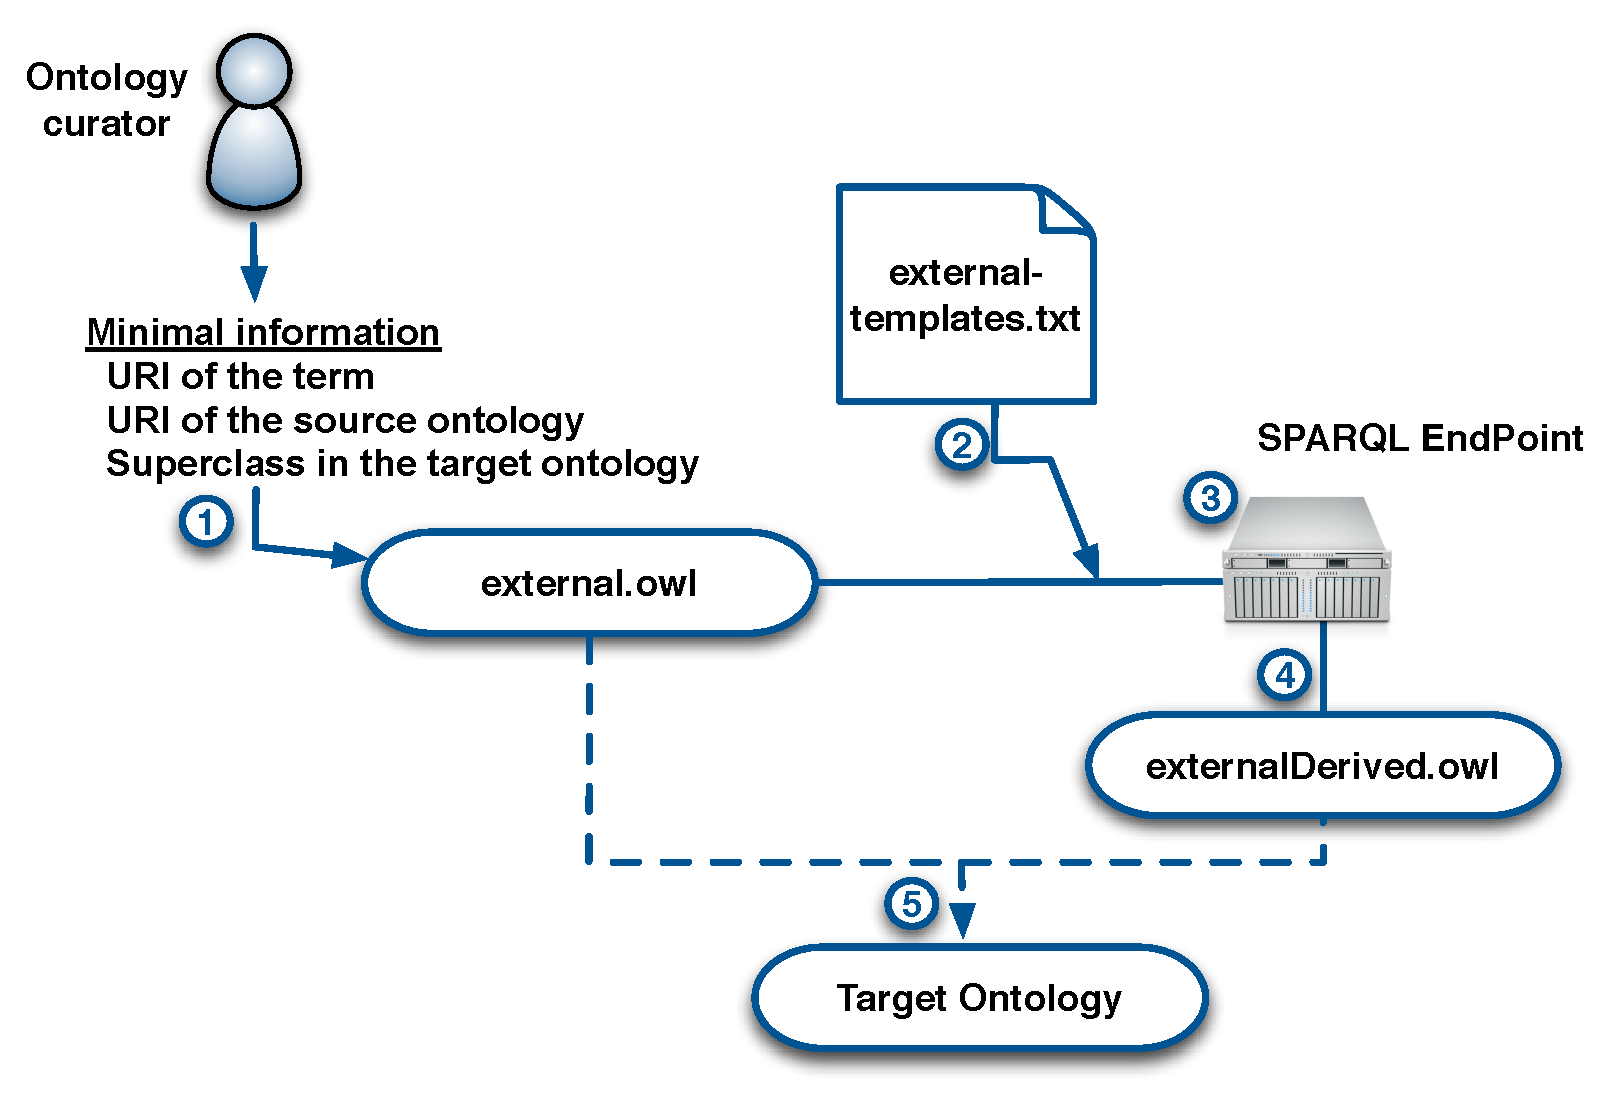
\includegraphics[width=.9\linewidth]{./figs/mechanism2.pdf}
}
\caption{Diagram of the MIREOT mechanism.
1. The ontology editor gathers the minimal information for the class to import and adds it into the external.owl file
2. A script parses the external.owl file, and for each class selects the appropriate SPARQL CONSTRUCT template.
3. The SPARQL query is executed against a SPARQL endpoint (\emph{e.g.}, Neurocommons)
4. The results of the SPARQL queries are combined into the externalDerived.owl file
5. The target ontology imports the external.owl and externalDerived.owl files.
}
\label{fig:mechanism2}
\end{figure}




\subsection{Use Case One - Basophil and Cell classes}

We replaced the \ac{OBI} $cell$ class with that from the \ac{CL} ontology~\citep{CL}. 
\ac{CL} is part of the \ac{OBO} Foundry effort, and we would like to use the $cell$ class as defined by this resource, instead of creating an other class denoting the same entity.
This class can then be used in turn to import other classes as needed.
For example the following invocation of the \emph{add-to-external.pl} script:

\begin{footnotesize}
\begin{verbatim}
perl add-to-external.pl CL:0000767 CL:0000000 
\end{verbatim}
\end{footnotesize}

will add the class $basophil$ (CL:0000767) as subclass of the class $cell$  (CL:0000000), and set the source ontology URI as \url{http://purl.org/obo/owl/CL}.
Once imported, the $basophil$ and $cell$ classes can be used like any other OBI class. For example, the process $electroporation$ is defined as:

\begin{footnotesize}
\begin{verbatimtab}
Class: electroporation
      SubClassOf: 'cell permeabilization'
                              and has_specified_input some cell
                              and has_participant some 'power supply'
\end{verbatimtab}
\end{footnotesize}

More generally, additional axioms may be used to relate members of the class to other entities in the ontology.


\subsection{Use Case Two - taxonomic information}

The \textit{cell} use-case highlights what is likely to be the most common import scenario, \emph{i.e.}, a simple import of one external term, making it available for direct use in the target ontology.
However, in some cases, we may require more than that single external term, and to account for this \ac{MIREOT} has been devised to be flexible.

Consider the scenario in which we have two experiments, one in human and one in mouse. 
The files are annotated with the classes human and mouse from the ontology, which are in turn mapped from the NCBI taxonomy. 
We can easily imagine that somebody would want to have a query for all 
experiments in mammals, without specifying the exact species. In this case, we would need to know that human and mouse are 
subclasses (even indirect) of mammals in the NCBI taxonomy. The root term of the NCBI taxonomy is an example of term we didn't want to include in the \ac{OBI}, as it includes \textit{viroids}, \textit{unclassified sequences} and \textit{others sequences}, which we didn't consider useful when defining organisms.  Therefore, when mapping 
towards an NCBI term, we decided to retrieve all its superclasses as well up to specific levels (\textit{Archaea}, \textit{Bacteria}, \textit{Eukaryota} and \textit{Viruses}) of the 
NCBI taxonomy. 

When the \emph{create-external-derived.lisp} script parses the \emph{external.owl} file and encounters an NCBI taxonomy ID, it will therefore invoke a specific SPARQL query (cf figure \ref{fig:sparql2}). 
As per the mechanism described above, the minimum information about the imported external class (\emph{e.g.}, \emph{Mus musculus}) is defined in \emph{external.owl}, whereas the additional information (rank information - genus, kingdom, phylum, etc.- \emph{i.e.}, its  superclasses) is stored in \emph{ externalDerived.owl}.
On the same model, any information that the importing ontology editors would require could be added in the \emph{externalDerived.owl} file: the only requirement is to write the corresponding SPARQL query.

\subsection{Use Case Three - Unit instances}

Finally, the most recent use case addresses the needs for \ac{OBI} to represent units. The \ac{UO}~\citep{PATO} tackles this effort, and currently encompasses more than 2000 classes. 
However, the representation of units as classes doesn't comply with the design pattern chosen by \ac{OBI} and the \ac{IAO}, which take the stance that in the absence of a satisfactory unit representation theory, we should represent things we understand, \emph{i.e.}, unit labels. 
We therefore decided on importing the \ac{UO} classes corresponding to specific units (such as \textit{gram} or \textit{meter}) as instances of the \ac{IAO} class \textit{measurement unit label}.
The figure \ref{fig:protege} shows the result of this addition into the \ac{OBI} hierarchy.

\begin{figure}[t]
\centering
{
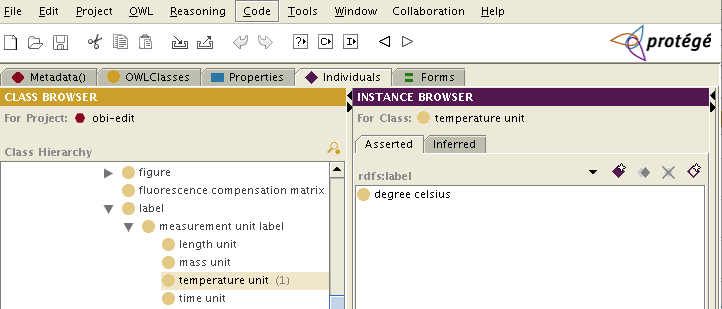
\includegraphics[width=.9\linewidth]{./figs/protege.png}
}
\caption{Screenshot of the Protege editor showing the class \textit{temperature unit} and its instance \textit{degree celsius}, as imported using the \ac{MIREOT} mechanism from the \ac{UO} ontology.
}
\label{fig:protege}
\end{figure}

We currently are in contact with the developers of the \ac{UO} to reach agreement on the best way to represent unit in a consistent manner, and we expect to align the different resources as part of the \ac{OBO} Foundry collaborative effort.


\begin{figure}[t]
\scriptsize
\verbatiminput{./figs/sparql2.txt} 
\caption{Template SPARQL query for import from the NCBI taxonomy. The \_ID\_GOES\_HERE\_ pattern will be replaced by the relevant NCBITax ID dynamically via script when building the CONSTRUCT query. This query allows retrieval of the class of interest and its parents up to a set of defined root classes. Note that the graph <http://purl.org/science/graph/obo/NCBITaxon> contains the source ontology, but the full store includes inferred subClassOf triples.}
\label{fig:sparql2}
\end{figure}




\section{Discussion}

The MIREOT mechanism offers a lightweight mechanism for importing specific classes from external ontologies. The approach is decoupled from the importing ontology, allowing a computational update mechanism which does not interfere with the primary ontology under development.

\ac{MIREOT} is currently implemented and used by several ontology efforts, including \ac{OBI}, the \ac{IAO}, the \ac{VO}~\citep{VO}, the \ac{IDO}~\citep{IDO} and the \ac{InfluenzO}~\citep{InfluenzO}.
In the context of \ac{OBI}, 472 terms are currently explicitly imported, which in turn leads to actual integration of 1447 classes (due to the automatic retrieval of parents when using the NCBI taxonomy). 



With broader use of the MIREOT mechanism by OBI and other resources, several minor issues arose.
For example, consider the case of \ac{IAO} developers requiring import of the term $investigation$.  This class already exists in \ac{OBI}, and \ac{IAO} developers therefore chose to MIREOT it, effectively integrating the class \url{http://purl.obolibrary.org/obo/OBI_0000066} and distributing it as part of the \ac{IAO} releases.
However, \ac{OBI} imports \ac{IAO}, and therefore re imports, \emph{via IAO}, its own $investigation$ class. This is not problematic in general, redundancy of information in OWL files being of no consequence. However when \ac{OBI} curators decided to update the definition of the $investigation$ class, the information natively in \ac{OBI} and that imported from \ac{IAO} became out-of-sync: two different definitions were displayed to the curators. Moreover one of them could not be edited as it is outside the remit of OBI to edit IAO definitions.

One solution to this problem would be to update the \ac{IAO} import - but this requires a release of \ac{OBI} with the updated $investigation$ definition, its upload on Neurocommons, and for the \ac{IAO} developers to update their information and produce a new release of \ac{IAO}. At best, this implies a delay of a few days, more realistically of a few weeks until the information in both files is again synchronized.
A better solution would be for tools to recognize and prioritize the origin of a class based on its URI. Ontology editing tools would display only the information originating from the target ontology when editing the target ontology file.
Such a solution also has consequences; when updating the information from the SPARQL endpoint, a specification of which \ac{RDF} graph~\citep{RDF} the term \emph{originally} belonged to is required. Taking again the example of the $investigation$ class, when querying based on its URI without specifying the RDF graph, the \ac{OBI} class, but also the one distributed by \ac{IAO}, will be returned, which is not the desired behavior; in our example, the \ac{IAO} annotation property values are now out of date compared to the original and authoritative \ac{OBI} file. 

Finally, when updating MIREOTed information, the SPARQL endpoint where the information resides must be up-to-date. The implementation currently relies on the \ac{OBO} Foundry resources at the Neurocommons \ac{OBO} distribution. This is updated nightly with the latest information from the \ac{OBO} server, and can therefore be reasonably relied upon for accessing current resources. The timeliness of the information may not always be known if extending the mechanism to another SPARQL endpoint, or other sets of ontological resources.

The \ac{MIREOT} standard presents an approach to importing classes from external ontologies that removes the overhead of full ontology imports whilst maintaining a decoupled but usable reference to the external classes. There is a clear trade-off that \ac{MIREOT} offers between practicality and full, axiomatic completeness. By importing only the desired parts of an external ontology there is the risk that inferences drawn may be incomplete or incorrect; correct inference using the external classes is only guaranteed if the full ontology, or a module, is imported. It does however present the important advantage of overcoming the obstacle presented by ontologies which are not fully interoperable at present.

Since only partial, reasoner-supported consistency checking is undertaken, extra care is taken when we need to make assertions about an imported term.

In adding axioms, such as the subclass axiom when importing the external term, the aim is to only assert true statements.
In our experience with the better OBO ontologies, the denotation of the term, as explained in the definition or documentation, is clearer and more correct than the axiomatization. 
If additional restrictions are required those should be stored in the importing ontology: the \emph{external.owl} and \emph{externalDerived.owl} are meant to include only the imported information.
It is anticipated that some of the statements added by the importing ontology may migrate to the source ontologies at some point in the future; a fruit of the collaborative nature of OBO Foundry ontology development.

When deciding to import an external term the textual definition is reviewed and, if required, discussion with the original editor is undertaken.
As we are importing from \ac{OBO} Foundry candidate ontologies we have a community process for monitoring change, a shared understanding of the basics of our domain, and the intention to eventually share the same upper-level ontology. 
Therefore, it is expected that terms will be deprecated if there is a significant change in meaning, and are flexible enough to adjust and update our import of terms as the other ontologies start enhancing their logical definitions.

\section{Future work}
The current implementation of the \ac{MIREOT} guidelines relies on command-line scripts, making it difficult for some curators to use. 
A web service, OntoFox~\citep{OntoFox}, has been developed by the He group at the University of Michigan to facilitate the process: ontology editors can use web forms to input their requirements, or submit specific OntoFox-formatted files for batch creation or update.
It is also expected that an option in the \ac{OBI} distribution will in the future enable the replacement of \emph{external.owl} with \emph{imports.owl}, a file of imports statements generated by extracting the ontology URIs mentioned in \emph{external.owl}. Users would then be able to import all of the external resources, therefore replacing the MIREOT selected terms.  As module extraction technology matures, we intend to include the ability to use such mechanisms for doing targeted imports, on a source-by-source basis.%

\section*{Acknowledgments}

In memory of our friend and colleague William Bug. 

The OBI consortium is (in alphabetical order): Ryan Brinkman, Bill Bug, Helen Causton, Kevin Clancy, Cristian Cocos, M\'elanie Courtot, Dirk Derom, Eric Deutsch, Liju Fan, Dawn Field, Jennifer Fostel, Gilberto Fragoso, Frank Gibson, Tanya Gray, Jason Greenbaum, Pierre Grenon, Jeff Grethe, Yongqun He, Mervi Heiskanen, Tina Hernandez-Boussard, Lawrence Hunter, Philip Lord, Allyson Lister, James Malone, Elisabetta Manduchi, Monnie McGee, Luisa Montecchi, Norman Morrison, Chris Mungall, Helen Parkinson, Bjoern Peters, Matthew Pocock, Philippe Rocca-Serra, Daniel Rubin, Alan Ruttenberg, Susanna-Assunta Sansone, Richard Scheuermann, Daniel Schober, Barry Smith, Larisa Soldatova, Holger Stenzhorn, Chris Stoeckert, Chris Taylor, Jessica Turner, John Westbrook,  Joe White, Trish Whetzel, Stefan Wiemann, Jie Zheng. 
The author's work is partially supported by funding from the NIH(R01EB005034),  the Public Health Agency of Canada / Canadian Institutes of Health Research Influenza Research Network (PCIRN), the EC EMERALD project (LSHG-CT-2006-037686), the BBSRC(BB/C008200/1, BB/D524283/1, BB/E025080/1), the EU FP7 DebugIT project (ICT-2007.5.2-217139), and the Michael Smith Foundation for Health Research.

\begin{thebibliography}{}

\bibitem[\protect\citeauthoryear{Bard et al.}{2005}]{CL} Bard J., Rhee S. Y., and Ashburner M. An ontology for cell types. \textit{Genome biology}, 6(2):R21, 2005. 

\bibitem[\protect\citeauthoryear{Degtyarenko et al.}{2008}]{ChEBI} Degtyarenko, K., de Matos, P., Ennis, M., Hastings, J., Zbinden, M., McNaught, A., Alcantara, R., Darsow, M., Guedj, M. and Ashburner, M. (2008) ChEBI: a database and ontology for chemical entities of biological interest. \textit{Nucleic Acids Res.} 36, D344-D350.

\bibitem[\protect\citeauthoryear{Gene Ontology Consortium}{2004}]{GO}
Gene Ontology Consortium. The gene ontology (go) database and informatics resource, \textit{Nucleic acids research} 32(90001), D258-D261.

\bibitem[\protect\citeauthoryear{GO editorial style guide}{}]{GOGuide} GO editorial style guide. Retrieved December 2, 2009, from \url{http://www.geneontology.org/GO.usage.shtml}.

\bibitem[\protect\citeauthoryear{Golbreich et al.}{2006}]{FMA} Golbreich C., Zhang S., and Bodenreider O.. The foundational model of anatomy in owl: Experience and perspectives. \textit{Web semantics (Online)}, 4(3):181-195, 2006. 

\bibitem[\protect\citeauthoryear{Grau et al.}{2007}]{Grau} Grau B.C., Horrocks I., Kazakov Y., and Sattler U. Extracting Modules from Ontologies: A Logic-based Approach. \textit{Proc. of the Third OWL Experiences and Directions Workshop}, number 258 in CEUR

\bibitem[\protect\citeauthoryear{Grau et al.}{2007}]{Grau2} Grau B.C., Horrocks I., Kazakov Y. and Sattler U. Just the right amount: Extracting modules from ontologies.\textit{In proc. of the 16th International World Wide Web Conference (WWW 2007)}

\bibitem[\protect\citeauthoryear{Grenon et al.}{2004}]{BFO} Grenon P., Smith B., and Goldberg L.. Biodynamic ontology: applying bfo in the biomedical domain. \textit{Studies in health 
technology and informatics}, 102:20-38, 2004. 

\bibitem[\protect\citeauthoryear{Haendel et al.}{2008}]{CARO} Haendel M.A., Neuhaus F., Osumi-Sutherland D., M. Mabee P., Mejino Jr. J.L.V., Mungall C.J., Smith B.. CARO - The Common Anatomy Reference Ontology, in \textit{Anatomy Ontologies for Bioinformatics Principles and Practice, Series: Computational Biology} , Vol. 6, ed. Burger, Albert; Davidson, Duncan; Baldock, Richard

\bibitem[\protect\citeauthoryear{Horrocks et al.}{2006}]{Horrocks} Horrocks I., Kutz O., and Sattler U. The Even More Irresistible SROIQ. \textit{In Proc. of the 10th Int. Conf. on Principles of Knowledge Representation and Reasoning (KR 2006)}, pages 57-67. AAAI Press, 2006.

\bibitem[\protect\citeauthoryear{Jimenez-Ruiz et al.}{2008}]{Jimenez} Jimenez-Ruiz E., Grau B.C., Sattler U., Schneider T. and Berlanga R. Safe and Economic Re-Use of Ontologies: A Logic-Based Methodology and Tool Support. \textit{5th European Semantic Web Conference (ESWC 2008)} 

\bibitem[\protect\citeauthoryear{Neurocommons OBO SPARQL endpoint}{}]{NeurocommonsSparql} Neurocommons OBO SPARQL endpoint. Retrieved December 2, 2009, from |url{http://sparql.obo.neurocommons.org/}.

\bibitem[\protect\citeauthoryear{OBI Ontology}{}]{OBI} OBI Ontology. Retrieved December 2, 2009, from \url{http://purl.obolibrary.org/obo/obi}.

\bibitem[\protect\citeauthoryear{OBI scripts}{2008}]{OBIScripts} OBI scripts. Retrieved December 2, 2009, from \url{http://purl.obolibrary.org/obo/obi/repository/}.

\bibitem[\protect\citeauthoryear{OntoFox webserver}{2009}]{OntoFox} OntoFox. Retrieved December 2, 2009, from \url{http://ontofox.hegroup.org/}.

\bibitem[\protect\citeauthoryear{Phenotypic Quality Ontology website}{}]{PATO} Phenotypic Quality Ontology. Retrieved December 2, 2009, from \url{http://obofoundry.org/wiki/index.php/PATO:Main_Page}

\bibitem[\protect\citeauthoryear{Seidenberg, Rector}{2006}]{Seidenberg} Seidenberg J., Rector A. Web ontology segmentation: analysis, classification and use. \textit{In proc. of the 15th International World Wide Web Conference (WWW 2006)}

\bibitem[\protect\citeauthoryear{Sirin et al.}{2007}]{Sirin}
 Sirin, E., Parsia, B., Grau, B. C., Kalyanpur, A., and Katz, Y. (2007). Pellet: A practical OWL-DL reasoner. \textit{Web Semant.}5, 51-53. 
 
 \bibitem[\protect\citeauthoryear{Smith et al.}{2007}]{OBOFoundry} Smith B., Ashburner M., Rosse C., Bard J., Bug W., Ceusters W., Goldberg L. J., Eilbeck K.,Ireland A., Mungall C. J., OBI Consortium, Leontis N., Rocca-Serra P., Ruttenberg A., Sansone S. A., Scheuermann R. H., Shah N., Whetzel P. L., and Lewis S. The obo foundry: coordinated evolution of ontologies to support biomedical data integration. \textit{Nature biotechnology}, 25(11):1251-1255, Nov 2007. 
 
 \bibitem[\protect\citeauthoryear{Smith et al.}{2004}]{OWL} Smith, M.K.; Welty C., McGuinness D.L., OWL Web Ontology Language Guide. Retrieved December 2, 2009, from \url{http://www.w3.org/2007/OWL/}.
 
  \bibitem[\protect\citeauthoryear{SPARQL queries template file}{2008}]{OBIQueries} SPARQL queries template file. Retrieved December 2, 2009, from \url{http://obi.svn.sourceforge.net/svnroot/obi/trunk/src/tools/build/external-templates.txt}
  
 \bibitem[\protect\citeauthoryear{SPARQL Query Language }{}]{SPARQL} SPARQL Query Language for RDF. Retrieved December 2, 2009, from \url{http://www.w3.org/TR/rdf- sparql- query/}. 
 
 \bibitem[\protect\citeauthoryear{RDF/XML Syntax Specification}{}]{RDF} RDF/XML Syntax Specification. Retrieved December 2, 2009, from \url{http://www.w3.org/TR/rdf-syntax-grammar/}
 
 \bibitem[\protect\citeauthoryear{Ruttenberg et al.}{2009}]{Neurocommons} Ruttenberg A, Rees J, Samwald M, Marshall M. Life sciences on the Semantic Web: the Neurocommons and beyond \textit{Briefings in Bioinformatics} 10 , 193-204 2009
 
 \bibitem[\protect\citeauthoryear{IDO website}{}]{IDO} The Infectious Disease Ontology. Retrieved December 2, 2009, from \url{http://www.infectiousdiseaseontology.org/}
 
 \bibitem[\protect\citeauthoryear{InfluenzO website}{}]{InfluenzO} The Influenza Ontology. Retrieved December 2, 2009, from \url{https://sourceforge.net/projects/influenzo/}.
 
 \bibitem[\protect\citeauthoryear{IAO website}{2008}]{IAO} The Information Artifact Ontology (IAO). Retrieved December 2, 2009, from \url{http://code.google.com/p/information- artifact- ontology/}.
 
 \bibitem[\protect\citeauthoryear{The Prot\'{e}g\'{e} Ontology Editor}{}]{Protege} The Prot\'{e}g\'{e} Ontology Editor and Knowledge Acquisition System. Retrieved December 2, 2009, from \url{http://protege.stanford.edu/}
 
 \bibitem[\protect\citeauthoryear{VO website}{}]{VO} The Vaccine Ontology. Retrieved December 2, 2009, from \url{http://www.violinet.org/vaccineontology/}

 \bibitem[\protect\citeauthoryear{Wheeler et al.}{2005}]{NCBI}
Wheeler D. L. , Barrett T., Benson D. A. , Bryant S. H., Canese K., Church D. M., DiCuccio M., Edgar R., Federhen S., 
 Helmberg W., Kenton D. L., Khovayko O., Lipman D. J., Madden T. L., Maglott D. R., Ostell J., Pontius J. U., Pruitt K. D., 
 SchulerG. D., Schriml L. M., Sequeira E., Sherry S. T., Sirotkin K., Starchenko G., Suzek T. O., Tatusov R., Tatusova T. A., 
 Wagner L., and Yaschenko E.. Database resources of the national center for biotechnology information. \textit{Nucleic acids 
research, } 33(Database issue), D39-45.

 
\end{thebibliography}
    
\begin{acronym}
\acro{BFO}{Basic Formal Ontology}
\acro{ChEBI}{Chemical Entities of Biological Interest}
\acro{CL}{Cell Type}

\acro{GO}{Gene Ontology}

\acro{MIREOT}{Minimum Information to Reference an External Ontology Term}

\acro{OBI}{Ontology of Biomedical Investigations}
\acro{OBO}{Open Biomedical Ontologies}
\acro{OWL}{Web Ontology Language}
\acro{IAO}{Information Artifact Ontology}
\acro{VO}{Vaccine Ontology}
\acro{IDO}{Infectious Disease Ontology}
\acro{InfluenzO}{Influenza Ontology}
\acro{CARO}{Common Anatomy Reference Ontology}
\acro{PRO}{Protein Ontology}
\acro{RDF}{Resource Description Framework}
\acro{FMA}{Foundational Model of Anatomy}
\acro{PATO}{Phenotypic Quality Ontology}
\acro{URI}{Uniform Resource Identifier}
\acro{UO}{Unit Ontology}
\end{acronym}




\end{document}
